% -*- TeX -*-
\documentclass[aspectratio=169]{beamer}

\usepackage{listings}

\usepackage{bm}
\usepackage{amsmath}
\usepackage{tikz}

\usetikzlibrary{decorations.pathreplacing}
\usetikzlibrary{fit,matrix}

\title{Crustal Deformation Modeling Tutorial}
\subtitle{Spontaneous Rupture with PyLith}
\author{Brad Aagaard \\
  Matthew Knepley \\
  Charles Williams}
\institute{
\includegraphics[scale=0.4]{../../logos/cig_blackfg}}
\date{June 27, 2017}


% ---------------------------------------------------- CUSTOMIZATION
%\newcommand{\thispdfpagelabel}[1]{}
\usetheme{CIG}

% Style information for PyLith presentations.

% Colors
\definecolor{ltorange}{rgb}{1.0, 0.74, 0.41} % 255/188/105
\definecolor{orange}{rgb}{0.96, 0.50, 0.0} % 246/127/0

\definecolor{ltred}{rgb}{1.0, 0.25, 0.25} % 255/64/64
\definecolor{red}{rgb}{0.79, 0.00, 0.01} % 201/0/3

\definecolor{ltpurple}{rgb}{0.81, 0.57, 1.00} % 206/145/255
\definecolor{purple}{rgb}{0.38, 0.00, 0.68} % 97/1/175

\definecolor{ltblue}{rgb}{0.2, 0.73, 1.0} % 51/187/255
\definecolor{mdblue}{rgb}{0.28, 0.50, 0.80} % 72/128/205
\definecolor{blue}{rgb}{0.12, 0.43, 0.59} % 30/110/150

\definecolor{ltltgreen}{rgb}{0.7, 1.00, 0.7} % 96/204/14
\definecolor{ltgreen}{rgb}{0.37, 0.80, 0.05} % 96/204/14
\definecolor{green}{rgb}{0.23, 0.49, 0.03} % 59/125/8
  
\definecolor{dkslate}{rgb}{0.18, 0.21, 0.28} % 47/53/72
\definecolor{mdslate}{rgb}{0.45, 0.50, 0.68} % 114/127/173
\definecolor{ltslate}{rgb}{0.85, 0.88, 0.95} % 216/225/229


\newcommand{\includefigure}[2][]{{\centering\includegraphics[#1]{#2}\par}}
\newcommand{\highlight}[1]{{\bf\usebeamercolor[fg]{structure}#1}}
\newcommand{\important}[1]{{\color{red}#1}}
\newcommand{\issue}[2]{\item[Issue:] {\color{red}#1}\\{\item[Soln:] \color{blue}#2}\\[4pt]}

\setbeamercolor{alerted text}{fg=ltgreen}
\setbeamertemplate{description item}[align left]


\newcommand{\lhs}[1]{{\color{blue}#1}}
\newcommand{\rhs}[1]{{\color{red}#1}}
\newcommand{\annotateL}[2]{%
  {\color{blue}\underbrace{\color{blue}#1}_{\color{blue}\mathclap{#2}}}}
\newcommand{\annotateR}[2]{%
  {\color{red}\underbrace{\color{red}#1}_{\color{red}\mathclap{#2}}}}
\newcommand{\eqnannotate}[2]{%
  {\color{blue}%
  \underbrace{\color{black}#1}_{\color{blue}\mathclap{#2}}}}

\newcommand{\trialvec}[1][]{{\vec{\psi}_\mathit{trial}^{#1}}}
\newcommand{\trialscalar}[1][]{{\psi_\mathit{trial}^{#1}}}
\newcommand{\basisvec}[1][]{{\vec{\psi}_\mathit{basis}^{#1}}}
\newcommand{\basisscalar}[1][]{{\psi_\mathit{basis}^{#1}}}

\newcommand{\tensor}[1]{\bm{#1}}
\DeclareMathOperator{\Tr}{Tr}

\usefonttheme[onlymath]{serif}

% minted shortcuts
\newminted{cfg}{bgcolor=ltslate,autogobble,fontsize=\tiny}
\newminted{bash}{bgcolor=ltltgreen,autogobble,fontsize=\tiny}

% PyLith components
\newcommand{\pylith}[1]{{\ttfamily\color{magenta}#1}}



% ========================================================= DOCUMENT
\begin{document}

% ------------------------------------------------------------ SLIDE
\maketitle

% ------------------------------------------------------------ SLIDE
\logo{
\includegraphics[height=4.5ex]{../../logos/cig_blackfg}}

% ========================================================== SECTION
\section{Introduction}

% ------------------------------------------------------------ SLIDE
\begin{frame}
  \frametitle{Concepts Covered in this Session}
  \summary{}

  \begin{itemize}
  \item Quasistatic simulations with spontaneous fault rupture driven
    by aseismic creep
  \item Fault constitutive models
    \begin{itemize}
    \item Slip-weakening
    \item Dieterich-Ruina rate-state friction w/ageing law
    \end{itemize}
  \item Nonlinear solver parameters
  \item Initial fault traction perturbations
  \end{itemize}

\end{frame}


% ========================================================== SECTION
\section{Implementation}
\subsection{Governing Equations}

% ------------------------------------------------------------ SLIDE
\begin{frame}[fragile]
  \frametitle{Fault Interface}
  \summary{Fault tractions couple deformation across interface}

  \begin{center}
    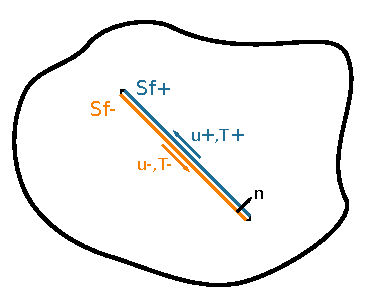
\includegraphics[height=7.0cm]{figs/domaindecomp}
  \end{center}

\end{frame}


% ------------------------------------------------------------ SLIDE
\begin{frame}[fragile]
  \frametitle{Governing Equations}
  \summary{Terms in governing equation associated with fault}

  \begin{itemize}
  \item Tractions on fault surface are analogous to boundary tractions
    \tikz{
      \matrix [matrix of nodes, ampersand replacement=\&] {
      \node {$ \displaystyle \ldots $}; \&
      \node [below delimiter=\}] {$ \displaystyle + \int_{S_T} \vec{\phi} \cdot \vec{T} \, dS$}; \&
      \node [below delimiter=\}] {$ \displaystyle - \int_{S_{f^+}} \vec{\phi} \cdot \vec{l} \, dS$}; \&
      \node [below delimiter=\}] {$ \displaystyle + \int_{S_{f^-}} \vec{\phi} \cdot \vec{l} \, dS$}; \&
      \ldots = 0 \\
      \& \node {Neumann BC}; \& 
      \node {Fault +}; \&
      \node {Fault -}; \& \\
    };
}
  \item Relationship between slip and relative displacement
    \tikz{
      \matrix [matrix of nodes, ampersand replacement=\&] {
        \node {$ \displaystyle \int_{S_f} \vec{\phi} \cdot ($}; \&
        \node [below delimiter=\}] {$\displaystyle\vec{d}$}; \&
        \node {$ \displaystyle - $}; \&
        \node [below delimiter=\}] {$ \displaystyle (\vec{u}_{+} - \vec{u}_{-}) $}; \&
        \node {$ \displaystyle ) dS = 0 $}; \\
        \& Slip \& \& Relative Disp. \& \\
    };
}
  \end{itemize}

\end{frame}


% ------------------------------------------------------------ SLIDE
\begin{frame}
  \frametitle{Fault Constitutive Model}
  \summary{Fault constitutive model places constraints on Lagrange multipliers}

  \begin{itemize}
  \item Shear components of Lagrange multipliers limited by fault
    constitutive model
    \begin{equation}
      l_\mathit{shear} \leq T_\mathit{friction}
    \end{equation}
  \item Fault friction depends on cohesion, coefficient of friction,
    and normal traction
    \begin{equation}
      T_\mathit{friction} = \left\{ \begin{array}{ll}
          T_\mathit{cohesion} - \mu_\mathit{f} T_\mathit{normal} &
          T_\mathit{normal} \leq 0 \\
          T_\mathit{cohesion} & T_\mathit{normal} > 0
        \end{array} \right.
    \end{equation}
  \item Compression $\Rightarrow$ no interpenetration, opening
    $\Rightarrow$ free surface
    \begin{equation}
      T_\mathit{normal} u_\mathit{normal} = 0 
    \end{equation}
  \end{itemize}
  
\end{frame}


% ------------------------------------------------------------ SLIDE
\begin{frame}
  \frametitle{Solution Algorithm}
  \summary{Solution requires ``friction sensitivity'' solve in
    addition to nonlinear solve}

  \begin{enumerate}
  \item Perform nonlinear iteration assuming no additional slip
  \item Check to see if fault constitutive model is satisfied
  \item If not satisfied, estimate slip required to reduce traction
    \begin{enumerate}
    \item Extract subset of system associated with the fault
      \begin{equation}
        \begin{pmatrix}
          \tensor{K}_{n^+n^+} & 0 & \tensor{L}_p^T  \\
          0 & \tensor{K}_{n^-n^-} & -\tensor{L}_p^T \\
          \tensor{L}_p & -\tensor{L}_p & 0
        \end{pmatrix}
        \begin{pmatrix}
          \vec{u}_{n^+} \\
          \vec{u}_{n^-} \\
          \vec{l}_p \\
        \end{pmatrix}
        =
        \begin{pmatrix}
          \vec{b}_{n^+} \\
          \vec{b}_{n^-} \\
          \vec{b}_p \\
        \end{pmatrix}
      \end{equation}
    \item Perturb Lagrange multipliers to satisfy friction criterion
    \item Inner solve to get slip producing Lagrange multiplier perturbation
      \vspace*{-2mm}
      \begin{gather}
        \tensor{K}_{n^+n^+} \cdot \partial \vec{u}_{n^+} = 
        - \tensor{L}_p^T \cdot \partial \vec{l}_p, \\
        \tensor{K}_{n^-n^-} \cdot \partial \vec{u}_{n^-} =
        \tensor{L}_p^T \cdot \partial \vec{l}_p, \\
        \partial \vec{d}_p =  \partial \vec{u}_{n^+} - \partial \vec{u}_{n^-}.        
      \end{gather}
    \end{enumerate}
  \item Repeat
  \end{enumerate}

\end{frame}


% ------------------------------------------------------------ SLIDE
\begin{frame}
  \frametitle{Coming in PyLith v3.x}
  \summary{New fault friction formulation}

  \begin{itemize}
  \item Change meaning of Lagrange multiplier for fault friction
  \item Recompute Jacobian when switching from locked to sliding
  \item No ``friction sensitivity'' solve required
  \item \highlight{Much faster convergence in nonlinear solve}
  \end{itemize}

\end{frame}


% ------------------------------------------------------------ SLIDE
\begin{frame}
  \frametitle{Friction and Nonlinear Solver Parameters}
  \summary{Solver tolerances are \important{very} important}

  \begin{itemize}
  \item Dynamic (spontaneous rupture) fault parameters
    \begin{description}
    \item[\property{zero\_tolerance}] Iterative solver is not exact,
      so need threshold to detect nucleation of slip.
    \item[\property{zero\_tolerance\_normal}] Suppress fault opening
      for near zero values of slip.
    \end{description}
  \item Linear solver must converge to tighter tolerance than fault
    \property{zero\_tolerance} for fault to ``lock''
    \begin{description}
    \item[\property{ksp\_rtol}] Set to very small value to force
      absolute convergence
    \item[\property{ksp\_atol}] Must be smaller than fault
      \property{zero\_tolerance}
    \end{description}
  \item Nonlinear solver tolerance should not be smaller than
    fault \property{zero\_tolerance}
    \begin{description}
    \item[\property{snes\_rtol}] Set to very small value to force
      absolute convergence
    \item[\property{snes\_atol}] Must be larger than fault
      \property{zero\_tolerance}
    \end{description}
  \end{itemize}    

\end{frame}


% ------------------------------------------------------------ SLIDE
\begin{frame}[fragile]
  \frametitle{Friction and Nonlinear Solver Parameters}
  \summary{Parameters from a typical example (see examples)}

  \begin{cfg}
<h>[pylithapp.problem.interfaces.fault]</h>
<p>zero_tolerance</p> = 1.0e-9
<p>zero_tolerance_normal</p> = 1.0e-9

<h>[pylithapp.petsc]</h>
# Linear solver tolerances
<p>ksp_rtol</p> = 1.0e-20
<p>ksp_atol>/p> = 1.0e-10

# Nonlinear solver tolerances
<p>snes_rtol</p> = 1.0e-20
<p>snes_atol</p> = 1.0e-8

# Set preconditioner for friction sensitivity solve
<p>friction_pc_type</p> = asm
<p>friction_sub_pc_factor_shift_type</p> = nonzero
\end{cfg}
    
\end{frame}


% ========================================================== SECTION
\subsection{Friction Models}

% ------------------------------------------------------------ SLIDE
\begin{frame}
  \frametitle{Fault Constitutive Models}
  \summary{PyLith contains some of the more popular fault
    constitutive models}

  \begin{tabular}{lp{3in}}
    {\bf\color{green} Static} & Constant coefficient of friction \\
    {\bf\color{green} Slip-Weakening} & Friction decreases with slip to a
    lower limit \\
    {\bf\color{green} Time-Weakening} & Time replaces slip in slip-weakening
    friction model \\
    {\bf\color{green} Rate-State} & Dieterich-Ruina rate-state friction with
    ageing law 
  \end{tabular}
  
  \vfill 
  Some additional, less popular, fault-constitutive models with
  combinations of slip-weakening and time-weakening are available for
  use in the SCEC Dynamic Rupture benchmarks. 
  \vfill

\end{frame}


% ------------------------------------------------------------ SLIDE
\begin{frame}
  \frametitle{Static Friction}
  \summary{Fault has constant coefficient of friction}

  \begin{itemize}
  \item Coefficient of friction
    \begin{equation}
      \mu_f = \mu_\mathit{static}
    \end{equation}
  \item Slip continues once threshold shear traction is reached
  \item No stick-slip behavior
  \item Generally only used in static simulations
  \end{itemize}
  
\end{frame}


% ------------------------------------------------------------ SLIDE
\begin{frame}
  \frametitle{Slip-Weakening Friction}
  \summary{Fault weakens with slip until it reaches a lower limit}

  \begin{equation}
    \mu_f = \left\{ \begin{array}{ll}
        \mu_\mathit{dynamic} + (1 - \frac{D}{D_0})
        (\mu_\mathit{static} -\mu_\mathit{dynamic}) & D \leq D_0 \\
        \mu_\mathit{dynamic} & D > D_0
      \end{array} \right.
  \end{equation}
  \begin{center}
    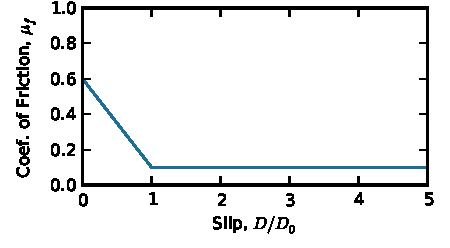
\includegraphics[height=1.65in]{figs/friction_slipweak}
  \end{center}
  
\end{frame}


% ------------------------------------------------------------ SLIDE
\begin{frame}
  \frametitle{Time-Weakening Friction}
  \summary{Fault weakens with time until it reaches a lower limit}
  
  \begin{equation}
    \mu_f = \left\{ \begin{array}{ll}
        \mu_\mathit{dynamic} + (1 - \frac{t}{t_0})
        (\mu_\mathit{static} -\mu_\mathit{dynamic}) & t \leq t_0 \\
        \mu_\mathit{dynamic} & t > t_0
      \end{array} \right.
  \end{equation}
  \begin{center}
    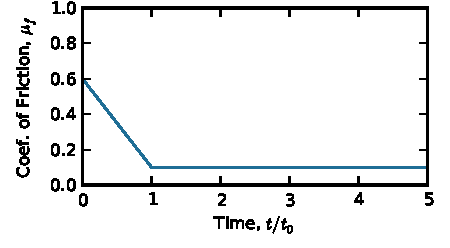
\includegraphics[height=1.65in]{figs/friction_timeweak}
  \end{center}
  
\end{frame}


% ------------------------------------------------------------ SLIDE
\begin{frame}
  \frametitle{Rate-State Friction with Ageing Law}
  \summary{Dieterich-Ruina rate-state friction with ageing evolution law}
  
  \begin{gather}
    \mu_f = \left\{ \begin{array}{ll}
        \mu_0 + a \ln (\frac{V}{V_0}) + b \ln (\frac{V_0 \theta}{L}) & V \ge V_\mathit{linear} \\
        \mu_0 + a \ln (\frac{V_\mathit{linear}}{V_0}) + b \ln
        (\frac{V_0\theta}{L}) - a (1 - \frac{V}{V_\mathit{linear}}) & V
        < V_\mathit{linear}
      \end{array} \right. \\
    \frac{d \theta}{dt} = 1 - \frac{V \theta}{L}
  \end{gather}
  \begin{center}
    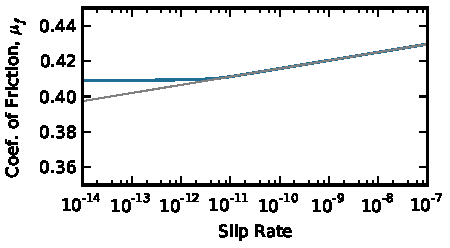
\includegraphics[height=1.65in]{figs/friction_ratestate}
  \end{center}
  
\end{frame}


% ========================================================== SECTION
\subsection{Parameters}

% ------------------------------------------------------------ SLIDE
\begin{frame}
  \frametitle{Spontaneous Rupture Parameters}
  \summary{Overview of principal components}
  
  \begin{tabular}{lp{3in}}
    \component{FaultCohesiveDyn} & Fault object for spontaneous rupture \\
    \component{FrictionModel} & Fault constitutive model \\
    \component{TractPerturbation} & Prescribed spatial and/or temporal variation in fault tractions \\
    \component{SolverNonlinear} & Quasi-static simulations with spontaneous rupture require nonlinear solver
  \end{tabular}
  
\end{frame}


% ------------------------------------------------------------ SLIDE
\begin{frame}[fragile]
  \frametitle{Spontaneous Rupture Parameters}
  \summary{Example of fault parameters in a {\tt .cfg} file}

\begin{cfg}
<h>[pylithapp.timedependent.interfaces]</h>
<f>fault</f> = pylith.faults.FaultCohesiveDyn

<h>[pylithapp.timedependent.interfaces.fault]</h>
<f>friction</f> = pylith.friction.StaticFriction
<p>friction.label</p> = Static friction

<f>friction.db_properties</f> = spatialdata.spatialdb.UniformDB
<p>friction.db_properties.label</p> = Static friction
<p>friction.db_properties.values</p> = [friction-coefficient,cohesion]
<p>friction.db_properties.data</p> = [0.6,0.0*Pa]

<f>traction_perturbation</f> = pylith.faults.TractPerturbation
<p>traction_perturbation.db_initial</p> = spatialdata.spatialdb.SimpleDB
<p>traction_perturbation.db_initial.label</p> = Initial fault tractions
<p>traction_perturbation.db_initial.iohandler.filename</p> = spatialdb/tractions.spatialdb
\end{cfg}
  
\end{frame}


% ========================================================== SECTION
\section{examples/2d/subduction}

% ------------------------------------------------------------ SLIDE
\begin{frame}
  \frametitle{Quasi-static Spontaneous Ruptures}
  \summary{}
  
  \important{Step 5 in {\tt examples/3d/subduction} does not work yet,
    and will likely take many minutes to run when it does work.}

  \vfill
  New examples in {\tt\color{red} examples/2d/subduction}. Earthquake
  cycle with spontaneous rupture driven by subducting slab.
  \vfill

  \begin{description}
  \item[{\tt Step05}] Slip-weakening friction
  \item[{\tt Step06}] Rate-state friction
  \end{description}
  
\end{frame}


% ------------------------------------------------------------ SLIDE
\begin{frame}
  \frametitle{2-D Subduction Zone Description}
  \summary{}

  \includefigure[height=7.0cm]{figs/subduction2d_diagram}
  
\end{frame}


% ------------------------------------------------------------ SLIDE
\begin{frame}[fragile]
  \frametitle{Step 5: Tour of Input Files}
  \summary{}

  \begin{description}
  \item[{\tt pylithapp.cfg}] Parameters (mostly) common to Steps 1--6
  \item[{\tt step05.cfg}] Parameters specific to Step 5
  \item[{\tt fault\_slabtop\_slipweakening.spatialdb}] Friction properties spatial database
  \item[{\tt fault\_slabtop\_tractions.spatialdb}] Fault tractions spatial database
  \end{description}

  \vfill

  Run the simulation:\\
  \important{\tt pylith step05.cfg $>$\& step05.log \&} \\
  {\tt tail -f step05.log}
  
\end{frame}


% ------------------------------------------------------------ SLIDE
\begin{frame}
  \frametitle{Step 5: Slip Profiles Versus Time}
  \summary{Earthquake rupture causes slip over entire fault}

  \includefigure[height=7.0cm]{figs/subduction2d_step05_slip}
  
\end{frame}


% ------------------------------------------------------------ SLIDE
\begin{frame}[fragile]
  \frametitle{Step 6: Tour of Input Files}
  \summary{}

  \begin{description}
  \item[{\tt step06.cfg}] Parameters specific to Step 5
  \item[{\tt fault\_slabtop\_ratestate.spatialdb}] Friction properties spatial database
  \end{description}

  \vfill

  Run the simulation:\\
  \important{\tt pylith step06.cfg $>$\& step05.log \&} \\
  {\tt tail -f step06.log}
  
\end{frame}


% ------------------------------------------------------------ SLIDE
\begin{frame}
  \frametitle{Step 6: Slip Profiles Versus Time}
  \summary{Earthquake rupture causes slip over entire fault}

  \includefigure[height=7.0cm]{figs/subduction2d_step06_slip}
  
\end{frame}


% ------------------------------------------------------------ SLIDE
\begin{frame}
  \frametitle{Spontaneous Rupture Tips}
  \summary{Fault friction is inherently highly nonlinear}

  \begin{itemize}
  \item Spontaneous rupture often localizes stresses, requiring very
    high resolution meshes around fault.
  \item Friction parameters from the laboratory are usually not
    numerically tractable.
  \item You often need to regularize the friction model to obtain
    numerically stable solutions.
    \begin{itemize}
    \item Increase slip/time over which friction coefficient
      evolves.
    \item Reduce difference between ``yield'' stress and sliding
      stress.
    \item Reduce time step and discretization size.
    \end{itemize}
  \end{itemize}

  \end{frame}


% ======================================================================
\end{document}


% End of file
